% -*- TeX-master: "sicp.tex" -*-

\section{Hierarchical Data and the Closure Property}
\label{sec:2.2}

As we have seen, pairs provide a primitive ``glue'' that we can use to
construct compound data objects.  Figure \ref{fig:2.2} shows a
standard way to visualize a pair -- in this case, the pair formed by
\scheme|(cons 1 2)|.  In this representation, which is called
\textit{box-and-pointer notation}, each object is shown as a
\textit{pointer} to a box.  The box for a primitive object contains a
representation of the object.  For example, the box for a number
contains a numeral.  The box for a pair is actually a double box, the
left part containing (a pointer to) the \scheme|car| of the pair and
the right part containing the \scheme|cdr|.


We have already seen that \scheme|cons| can be used to combine not
only numbers but pairs as well.  (You made use of this fact, or
should have, in doing exercises \ref{exc:2.2}
and \ref{exc:2.3}.)  As a consequence, pairs provide a universal
building block from which we can construct all sorts of data
structures.  Figure \ref{fig:2.3} shows two ways
to use pairs to combine the numbers 1, 2, 3, and 4.

\begin{figure}
\centering
%\begin{tikzpicture}
  % TODO: create the box and pointer diagram
%\end{tikzpicture}
\caption{Box-and-pointer representation of \verbatim(cons 1 2)|}
\label{fig:2.2}
\end{figure}

\begin{figure}
  \centering
  \placeholder
  \caption{Two ways to combine 1, 2, 3, and 4 using pairs}
  \label{fig:2.3}
\end{figure}

The ability to create pairs whose elements are pairs is the essence of
list structure's importance as a representational tool.  We refer to
this ability as the \textit{closure property} of \scheme|cons|.  In
general, an operation for combining data objects satisfies the closure
property if the results of combining things with that operation can
themselves be combined using the same operation.\footnote{6} Closure
is the key to power in any means of combination because it permits us
to create \textit{hierarchical} structures -- structures made up of
parts, which themselves are made up of parts, and so on.

From the outset of chapter 1, we've made essential use of closure in
dealing with procedures, because all but the very simplest programs
rely on the fact that the elements of a combination can themselves be
combinations.  In this section, we take up the consequences of closure
for compound data.  We describe some conventional techniques for using
pairs to represent sequences and trees, and we exhibit a graphics
language that illustrates closure in a vivid way.\footnote{7}


\subsection{Representing Sequences}
\label{sec:2.2.1}



\begin{figure}
  \centering
  % TODO: create the diagram
  \caption{The sequence 1, 2, 3, 4 represented as a chain of pairs.}
  \label{fig:2.3}
\end{figure}

One of the useful structures we can build with pairs is a
\textit{sequence} -- an ordered collection of data objects.  There
are, of course, many ways to represent sequences in terms of pairs.
One particularly straightforward representation is illustrated in
figure \ref{fig:2.4}, where the sequence 1, 2, 3, 4 is represented as
a chain of pairs.  The \scheme|car| of each pair is the corresponding
item in the chain, and the \scheme|cdr| of the pair is the next pair
in the chain.  The \scheme|cdr| of the final pair signals the end of
the sequence by pointing to a distinguished value that is not a pair,
represented in box-and-pointer diagrams as a diagonal line and in
programs as the value of the variable \scheme|nil|.  The entire
sequence is constructed by nested \scheme|cons| operations:

\begin{schemedisplay}
(cons 1
      (cons 2
            (cons 3
                  (cons 4 nil))))
\end{schemedisplay}


Such a sequence of pairs, formed by nested \scheme|cons|es, is called
a \textit{list}, and Scheme provides a primitive called \scheme|list|
to help in constructing lists.\footnote{8} The above sequence could be
produced by \scheme|(list 1 2 3 4)|.  In general,


\begin{schemedisplay}
(list <a_1> <a_2> ... <a_n>)
\end{schemedisplay}
is equivalent to


\begin{schemedisplay}
(cons <a_1> (cons <a_2> (cons \scheme|...| (cons <a_n> nil) ...)))
\end{schemedisplay}
Lisp systems conventionally print lists by printing the sequence of
elements, enclosed in parentheses.  Thus, the data object in
figure \ref{fig:2.4} is printed as \scheme|(1 2 3 4)|:


\begin{schemedisplay}
> (define one-through-four (list 1 2 3 4))

> one-through-four
(1 2 3 4)
\end{schemedisplay}
Be careful not to confuse the expression \scheme|(list 1 2 3 4)| with the
list \scheme|(1 2 3 4)|, which is the result obtained when the expression
is evaluated.  Attempting to evaluate the expression \scheme|(1 2 3 4)| will
signal an error when the interpreter tries to apply the procedure \scheme|1| to arguments \scheme|2|, \scheme|3|, and \scheme|4|.


We can think of \scheme|car| as selecting the first item in the list,
and of \scheme|cdr| as selecting the sublist consisting of all but the
first item.  Nested applications of \scheme|car| and \scheme|cdr| can
be used to extract the second, third, and subsequent items in the
list.\footnote{9} The constructor \scheme|cons| makes a list like the
original one, but with an additional item at the beginning.


\begin{schemedisplay}
> (car one-through-four)
1

> (cdr one-through-four)
(2 3 4)
> (car (cdr one-through-four))
2

> (cons 10 one-through-four)
(10 1 2 3 4)

> (cons 5 one-through-four)
(5 1 2 3 4)
\end{schemedisplay}
The value of \scheme|nil|, used to terminate the chain of pairs, can
be thought of as a sequence of no elements, the \textit{empty list}.
The word \textit{nil} is a contraction of the Latin word
\textit{nihil}, which means ``nothing.''\footnote{10}


\subsubsection*{List operations}


The use of pairs to represent sequences of elements as lists is
accompanied by conventional programming techniques for manipulating
lists by successively ``\scheme|cdr|ing down'' the lists.  For example,
the procedure \scheme|list-ref| takes as arguments a list and a number
\textit{n} and returns the \textit{n}th item of the list.  It is customary to
number the elements of the list beginning with 0.  The method for
computing \scheme|list-ref| is the following:

\begin{itemize}
\item For $n = 0$, \scheme|list-ref| should return the \scheme|car| of
  the list.

\item Otherwise, \scheme|list-ref| should return the $(n - 1)$st item
  of the \scheme|cdr| of the list.
\end{itemize}

\begin{schemedisplay}
(define (list-ref items n)
  (if (= n 0)
      (car items)
      (list-ref (cdr items) (- n 1))))
(define squares (list 1 4 9 16 25))

> (list-ref squares 3)
16
\end{schemedisplay}

Often we \scheme|cdr| down the whole list.  To aid in this, Scheme
includes a primitive predicate \scheme|null?|, which tests whether its
argument is the empty list.  The procedure \scheme|length|, which
returns the number of items in a list, illustrates this typical
pattern of use:

\begin{schemedisplay}
(define (length items)
  (if (null? items)
      0
      (+ 1 (length (cdr items)))))
(define odds (list 1 3 5 7))

> (length odds)
4
\end{schemedisplay}
The \scheme|length| procedure implements a simple recursive plan. The
reduction step is:

\begin{itemize}
\item The \scheme|length| of any list is 1 plus the \scheme|length| of
  the \scheme|cdr| of the list.
\end{itemize}

This is applied successively until we reach the base case:

\begin{itemize}
\item The \scheme|length| of the empty list is 0.
\end{itemize}

We could also compute \scheme|length| in an iterative style:

\begin{schemedisplay}
(define (length items)
  (define (length-iter a count)
    (if (null? a)
        count
        (length-iter (cdr a) (+ 1 count))))
  (length-iter items 0))
\end{schemedisplay}

Another conventional programming technique is to ``\scheme|cons| up'' an
answer list while \scheme|cdr|ing down a list, as in the procedure \scheme|append|, which takes two lists as arguments and combines their
elements to make a new list:

\begin{schemedisplay}
> (append squares odds)
(1 4 9 16 25 1 3 5 7)

> (append odds squares)
(1 3 5 7 1 4 9 16 25)
\end{schemedisplay}
\scheme|Append| is also implemented using a recursive plan.  To
\scheme|append| lists \scheme|list1| and \scheme|list2|, do the
following:

\begin{itemize}
\item If \scheme|list1| is the empty list, then the result is just
  \scheme|list2|.

\item Otherwise, \scheme|append| the \scheme|cdr| of \scheme|list1|
  and \scheme|list2|, and \scheme|cons| the \scheme|car| of
  \scheme|list1| onto the result:
\end{itemize}

\begin{schemedisplay}
(define (append list1 list2)
  (if (null? list1)
      list2
      (cons (car list1) (append (cdr list1) list2))))
\end{schemedisplay}

\begin{Exercise}
\label{exc:2.17}
Define a procedure \scheme|last-pair| that returns the list that contains only
the last element of a given (nonempty) list:

\begin{schemedisplay}
> (last-pair (list 23 72 149 34))
(34)
\end{schemedisplay}
\end{Exercise}

\begin{Exercise}
\label{exc:2.18}
Define a procedure \scheme|reverse| that takes a list as argument and
returns a list of the same elements in reverse order:

\begin{schemedisplay}
> (reverse (list 1 4 9 16 25))
(25 16 9 4 1)
\end{schemedisplay}
\end{Exercise}

\begin{Exercise}
\label{exc:2.19}
Consider the change-counting program of section \ref{sec:1.2.2}.  It
would be nice to be able to easily change the currency used by the
program, so that we could compute the number of ways to change a
British pound, for example.  As the program is written, the knowledge
of the currency is distributed partly into the procedure
\scheme|first-denomination| and partly into the procedure
\scheme|count-change| (which knows that there are five kinds of
U.S. coins).  It would be nicer to be able to supply a list of coins
to be used for making change.

We want to rewrite the procedure \scheme|cc| so that its second
argument is a list of the values of the coins to use rather than an
integer specifying which coins to use.  We could then have lists that
defined each kind of currency:

\begin{schemedisplay}
(define us-coins (list 50 25 10 5 1))
(define uk-coins (list 100 50 20 10 5 2 1 0.5))
\end{schemedisplay}
We could then call \scheme|cc| as follows:

\begin{schemedisplay}
> (cc 100 us-coins)
292
\end{schemedisplay}
To do this will require changing the program \scheme|cc| somewhat.  It
will still have the same form, but it will access its second argument
differently, as follows:

\begin{schemedisplay}
(define (cc amount coin-values)
  (cond ((= amount 0) 1)
        ((or (< amount 0) (no-more? coin-values)) 0)
        (else
         (+ (cc amount
                (except-first-denomination coin-values))
            (cc (- amount
                   (first-denomination coin-values))
                coin-values)))))
\end{schemedisplay}
Define the procedures \scheme|first-denomination|,
\scheme|except-first-denomination|, and \scheme|no-more?| in terms of
primitive operations on list structures.  Does the order of the list
\scheme|coin-values| affect the answer produced by \scheme|cc|?  Why
or why not?
\end{Exercise}

\begin{Exercise}
\label{exc:2.20}
The procedures \scheme|+|, \scheme|*|, and \scheme|list| take
arbitrary numbers of arguments. One way to define such procedures is
to use \scheme|define| with \textit{dotted-tail notation}.  In a
procedure definition, a parameter list that has a dot before the last
parameter name indicates that, when the procedure is called, the
initial parameters (if any) will have as values the initial arguments,
as usual, but the final parameter's value will be a \textit{list} of
any remaining arguments.  For instance, given the definition

\begin{schemedisplay}
(define (f x y . z) \textit{<body>})
\end{schemedisplay}
the procedure \scheme|f| can be called with two or more arguments.
If we evaluate

\begin{schemedisplay}
(f 1 2 3 4 5 6)
\end{schemedisplay}
then in the body of \scheme|f|, \scheme|x| will be 1, \scheme|y| will be
2, and \scheme|z| will be the list \scheme|(3 4 5 6)|.
Given the definition

\begin{schemedisplay}
(define (g . w) \textit{<body>})
\end{schemedisplay}
the procedure \scheme|g| can be called with zero or more arguments.
If we evaluate

\begin{schemedisplay}
(g 1 2 3 4 5 6)
\end{schemedisplay}
then in the body of \scheme|g|, \scheme|w| will be the
list \scheme|(1 2 3 4 5 6)|.\footnote{11}

Use this notation
to write a procedure \scheme|same-parity| that takes one or more integers
and returns a list of all the arguments that have the same even-odd
parity as the first argument.  For example,
\begin{schemedisplay}
> (same-parity 1 2 3 4 5 6 7)
(1 3 5 7)

> (same-parity 2 3 4 5 6 7)
(2 4 6)
\end{schemedisplay}
\end{Exercise}

\subsubsection*{Mapping over lists}


One extremely useful operation is to apply some transformation
to each element in a list and generate the list of results.
For instance, the following procedure scales each number in a list by
a given factor:

\begin{schemedisplay}
(define (scale-list items factor)
  (if (null? items)
      nil
      (cons (* (car items) factor)
            (scale-list (cdr items) factor))))
> (scale-list (list 1 2 3 4 5) 10)
(10 20 30 40 50)
\end{schemedisplay}

We can abstract this general idea and capture it as a common pattern
expressed as a higher-order procedure, just as in section
\ref{sec:1.3}.  The higher-order procedure here is called
\scheme|map|.  \scheme|Map| takes as arguments a procedure of one
argument and a list, and returns a list of the results produced by
applying the procedure to each element in the list:\footnote{12}

\begin{schemedisplay}
(define (map proc items)
  (if (null? items)
      nil
      (cons (proc (car items))
            (map proc (cdr items)))))

> (map abs (list -10 2.5 -11.6 17))
(10 2.5 11.6 17)

> (map (lambda (x) (* x x))
       (list 1 2 3 4))
(1 4 9 16)
\end{schemedisplay}
Now we can give a new definition of \scheme|scale-list| in terms of \scheme|map|:
\begin{schemedisplay}
(define (scale-list items factor)
  (map (lambda (x) (* x factor))
       items))
\end{schemedisplay}


\scheme|Map| is an important construct, not only because it captures a
common pattern, but because it establishes a higher level of
abstraction in dealing with lists.  In the original definition of
\scheme|scale-list|, the recursive structure of the program draws
attention to the element-by-element processing of the list.  Defining
\scheme|scale-list| in terms of \scheme|map| suppresses that level of
detail and emphasizes that scaling transforms a list of elements to a
list of results.  The difference between the two definitions is not
that the computer is performing a different process (it isn't) but
that we think about the process differently.  In effect, \scheme|map|
helps establish an abstraction barrier that isolates the
implementation of procedures that transform lists from the details of
how the elements of the list are extracted and combined.  Like the
barriers shown in figure \ref{fig:2.1}, this abstraction gives us the
flexibility to change the low-level details of how sequences are
implemented, while preserving the conceptual framework of operations
that transform sequences to sequences.  Section \ref{sec:2.2.3}
expands on this use of sequences as a framework for organizing
programs.

\begin{Exercise}
\label{exc:2.21}
The procedure \scheme|square-list| takes a list of numbers as argument
and returns a list of the squares of those numbers.

\begin{schemedisplay}
> (square-list (list 1 2 3 4))
(1 4 9 16)
\end{schemedisplay}

Here are two different definitions of \scheme|square-list|.  Complete
both of them by filling in the missing expressions:

\begin{schemedisplay}
(define (square-list items)
  (if (null? items)
      nil
      (cons <\textit{??}> <\textit{??}>)))
(define (square-list items)
  (map <\textit{??}> <\textit{??}>))
\end{schemedisplay}
\end{Exercise}

\begin{Exercise}
\label{exc:2.22}
Louis Reasoner tries to rewrite the first \scheme|square-list| procedure of
exercise \ref{exc:2.21} so that it evolves an iterative
process:

\begin{schemedisplay}
(define (square-list items)
  (define (iter things answer)
    (if (null? things)
        answer
        (iter (cdr things) 
              (cons (square (car things))
                    answer))))
  (iter items nil))
\end{schemedisplay}
Unfortunately, defining \scheme|square-list| this way produces the
answer list in the reverse order of the one desired.  Why?

Louis then tries to fix his bug by interchanging the arguments to
\scheme|cons|:

\begin{schemedisplay}
(define (square-list items)
  (define (iter things answer)
    (if (null? things)
        answer
        (iter (cdr things)
              (cons answer
                    (square (car things))))))
  (iter items nil))
\end{schemedisplay}
This doesn't work either.  Explain.
\end{Exercise}

\begin{Exercise}
\label{exc:2.23}
The procedure \scheme|for-each| is similar to \scheme|map|.  It takes
as arguments a procedure and a list of elements.  However, rather than
forming a list of the results, \scheme|for-each| just applies the
procedure to each of the elements in turn, from left to right.  The
values returned by applying the procedure to the elements are not used
at all -- \scheme|for-each| is used with procedures that perform an
action, such as printing.  For example,
\begin{schemedisplay}
(for-each (lambda (x) (newline) (display x))
          (list 57 321 88))
<i>57</i>
<i>321</i>
<i>88</i>
\end{schemedisplay}
The value returned by the call to \scheme|for-each| (not illustrated
above) can be something arbitrary, such as true.  Give an
implementation of \scheme|for-each|.
\end{Exercise}

\subsection{Hierarchical Structures}
\label{sec:2.2.2}

The representation of sequences in terms of lists generalizes
naturally to represent sequences whose elements may
themselves be sequences.  For example, we can regard the object
\scheme|((1 2) 3 4)| constructed by

\begin{schemedisplay}
(cons (list 1 2) (list 3 4))
\end{schemedisplay}
as a list of three items, the first of which is itself a list,
\scheme|(1 2)|.  Indeed, this is suggested by the form in which the
result is printed by the interpreter.  Figure \ref{fig:2.5} shows the
representation of this structure in terms of pairs.

\begin{schemeregion}
  \begin{figure}
    \centering
    % TODO: fill in this diagram
    \caption{Structure formed by \scheme|(cons (list 1 2) (list 3 4))|}
    \label{fig:2.5}
  \end{figure}
\end{schemeregion}

Another way to think of sequences whose elements are sequences is as
\textit{trees}.  The elements of the sequence are the branches of the
tree, and elements that are themselves sequences are subtrees.  Figure
\ref{fig:2.6} shows the structure in figure \ref{fig:2.5} viewed as a
tree.

\begin{figure}
  \centering
  % TODO: fill in this diagram
  \caption{The list structure in figure \ref{fig:2.5} viewed as a tree.}
  \label{fig:2.6}
\end{figure}

Recursion is a natural tool for dealing with tree structures, since we
can often reduce operations on trees to operations on their branches,
which reduce in turn to operations on the branches of the branches,
and so on, until we reach the leaves of the tree.  As an example,
compare the \scheme|length| procedure of section \ref{sec:2.2.1} with
the \scheme|count-leaves| procedure, which returns the total number of
leaves of a tree:


\begin{schemedisplay}
(define x (cons (list 1 2) (list 3 4)))

> (length x)
3
> (count-leaves x)
4

> (list x x)
(((1 2) 3 4) ((1 2) 3 4))

> (length (list x x))
2

> (count-leaves (list x x))
8
\end{schemedisplay}

To implement \scheme|count-leaves|, recall the recursive plan for computing
\scheme|length|:

\begin{itemize}
\item \scheme|Length| of a list \scheme|x| is 1 plus \scheme|length|
  of the \scheme|cdr| of \scheme|x|.

\item \scheme|Length| of the empty list is 0.
\end{itemize}

\scheme|Count-leaves| is similar.  The value for the empty list is the same:

\begin{itemize}
\item \scheme|Count-leaves| of the empty list is 0.
\end{itemize}

But in the reduction step, where we strip off the \scheme|car| of the
list, we must take into account that the \scheme|car| may itself be a
tree whose leaves we need to count.  Thus, the appropriate reduction
step is


\begin{itemize}
\item \scheme|Count-leaves| of a tree \scheme|x| is
  \scheme|count-leaves| of the \scheme|car| of \scheme|x| plus
  \scheme|count-leaves| of the \scheme|cdr| of \scheme|x|.
\end{itemize}

Finally, by taking \scheme|car|s we reach actual leaves, so we need
another base case:


\begin{itemize}
\item \scheme|Count-leaves| of a leaf is 1.
\end{itemize}

To aid in writing recursive procedures on trees, Scheme provides the
primitive predicate \scheme|pair?|, which tests whether its argument
is a pair.  Here is the complete procedure:\footnote{13}


\begin{schemedisplay}
(define (count-leaves x)
  (cond ((null? x) 0)  
        ((not (pair? x)) 1)
        (else (+ (count-leaves (car x))
                 (count-leaves (cdr x))))))
\end{schemedisplay}

\begin{Exercise}
\label{exc:2.24}
Suppose we evaluate the expression \scheme|(list 1 (list 2 (list 3 4)))|.
Give the result printed by the interpreter, the corresponding
box-and-pointer structure, and the interpretation of this as a tree
(as in figure \ref{fig:2.6}).
\end{Exercise}

\begin{Exercise}
\label{exc:2.25}
Give combinations of \scheme|car|s and \scheme|cdr|s that will pick 7 from
each of the following lists:

\begin{schemedisplay}
(1 3 (5 7) 9)

((7))

(1 (2 (3 (4 (5 (6 7))))))
\end{schemedisplay}
\end{Exercise}

\begin{Exercise}
\label{exc:2.26}
Suppose we define \scheme|x| and \scheme|y| to be two lists:

\begin{schemedisplay}
(define x (list 1 2 3))
(define y (list 4 5 6))
\end{schemedisplay}
What result is printed by the interpreter in response to evaluating
each of the following expressions:

\begin{schemedisplay}
(append x y)

(cons x y)

(list x y)
\end{schemedisplay}
\end{Exercise}

\begin{Exercise}
\label{exc:2.27}
Modify your \scheme|reverse| procedure of exercise \ref{exc:2.18} to
produce a \scheme|deep-reverse| procedure that takes a list as argument
and returns as its value the list with its elements reversed and with
all sublists deep-reversed as well.  For example,

\begin{schemedisplay}
(define x (list (list 1 2) (list 3 4)))

x
<i>((1 2) (3 4))</i>

(reverse x)
<i>((3 4) (1 2))</i>

(deep-reverse x)
<i>((4 3) (2 1))</i>
\end{schemedisplay}
\end{Exercise}

\begin{Exercise}
\label{exc:2.28}
Write a procedure \scheme|fringe| that takes as argument a tree
(represented as a list) and returns a list whose elements are all the
leaves of the tree arranged in left-to-right order.  For example,

\begin{schemedisplay}
(define x (list (list 1 2) (list 3 4)))

(fringe x)
<i>(1 2 3 4)</i>

(fringe (list x x))
<i>(1 2 3 4 1 2 3 4)</i>
\end{schemedisplay}
\end{Exercise}

\begin{Exercise}
\label{exc:2.29}
A binary mobile consists of two branches, a left branch and a right
branch.  Each branch is a rod of a certain length, from which hangs
either a weight or another binary mobile.  We can represent a binary
mobile using compound data by constructing it from two branches (for
example, using \scheme|list|):


\begin{schemedisplay}
(define (make-mobile left right)
  (list left right))
\end{schemedisplay}
A branch is constructed from a \scheme|length| (which must be a number)
together with a \scheme|structure|, which may be either a number
(representing a simple weight) or another mobile:


\begin{schemedisplay}
(define (make-branch length structure)
  (list length structure))
\end{schemedisplay}

% TODO: use enumerate
a.  Write the corresponding selectors \scheme|left-branch| and
\scheme|right-branch|, which return the branches of a mobile, and
\scheme|branch-length| and \scheme|branch-structure|, which return 
the components of a branch.

b.  Using your selectors, define a procedure \scheme|total-weight| 
that returns the total weight of a mobile.

c.  A mobile is said to be \textit{balanced} if the torque applied
by its top-left branch is equal to that applied by its top-right
branch (that is, if the length of the left rod multiplied by the
weight hanging from that rod is equal to the corresponding product for
the right side) and if each of the submobiles hanging off its branches
is balanced. Design a predicate that tests whether a binary mobile is
balanced.

d.  Suppose we change the representation of mobiles so that the
constructors are

\begin{schemedisplay}
(define (make-mobile left right)
  (cons left right))
(define (make-branch length structure)
  (cons length structure))
\end{schemedisplay}
How much do you need to change your programs to convert to the new
representation?
\end{Exercise}

\subsubsection*{Mapping over trees}

Just as \scheme|map| is a powerful abstraction for dealing with
sequences, \scheme|map| together with recursion is a powerful
abstraction for dealing with trees.  For instance, the
\scheme|scale-tree| procedure, analogous to \scheme|scale-list| of
section \ref{sec:2.2.1}, takes as arguments a numeric factor and a
tree whose leaves are numbers.  It returns a tree of the same shape,
where each number is multiplied by the factor.  The recursive plan for
\scheme|scale-tree| is similar to the one for \scheme|count-leaves|:

\begin{schemedisplay}
> (define (scale-tree tree factor)
    (cond ((null? tree) nil)
          ((not (pair? tree)) (* tree factor))
          (else (cons (scale-tree (car tree) factor)
                      (scale-tree (cdr tree) factor)))))
> (scale-tree (list 1 (list 2 (list 3 4) 5) (list 6 7))
              10)
(10 (20 (30 40) 50) (60 70))
\end{schemedisplay}

Another way to implement \scheme|scale-tree| is to regard the tree as
a sequence of sub-trees and use \scheme|map|.  We map over the
sequence, scaling each sub-tree in turn, and return the list of
results.  In the base case, where the tree is a leaf, we simply
multiply by the factor:

\begin{schemedisplay}
(define (scale-tree tree factor)
  (map (lambda (sub-tree)
         (if (pair? sub-tree)
             (scale-tree sub-tree factor)
             (* sub-tree factor)))
       tree))
\end{schemedisplay}
Many tree operations can be implemented by similar combinations of
sequence operations and recursion.


\label{exc:2.30}
Define a procedure \scheme|square-tree| analogous to the
\scheme|square-list| procedure of exercise \ref{exc:2.21}.  That is,
\scheme|square-list| should behave as follows:

\begin{schemedisplay}
> (square-tree
   (list 1
         (list 2 (list 3 4) 5)
         (list 6 7)))
(1 (4 (9 16) 25) (36 49))
\end{schemedisplay}
Define \scheme|square-tree| both directly (i.e., without using any
higher-order procedures) and also by using \scheme|map| and recursion.
\end{Exercise}

\begin{Exercise}
\label{exc:2.31}
Abstract your answer to exercise \ref{exc:2.30} to produce a procedure
\scheme|tree-map| with the property that \scheme|square-tree| could be
defined as

\begin{schemedisplay}
(define (square-tree tree) (tree-map square tree))
\end{schemedisplay}
\end{Exercise}

\begin{Exercise}
\label{exc:2.32}
We can represent a set as a list of distinct elements, and we can
represent the set of all subsets of the set as a list of lists.  For
example, if the set is \scheme|(1 2 3)|, then the set of all subsets
is \scheme|(() (3) (2) (2 3) (1) (1 3) (1 2) (1 2 3))|.  Complete the
following definition of a procedure that generates the set of subsets
of a set and give a clear explanation of why it works:
\begin{schemedisplay}
(define (subsets s)
  (if (null? s)
      (list nil)
      (let ((rest (subsets (cdr s))))
        (append rest (map <??> rest)))))
\end{schemedisplay}
\end{Exercise}

\subsection{Sequences as Conventional Interfaces}
\label{sec:2.2.3}

In working with compound data, we've stressed how data abstraction
permits us to design programs without becoming enmeshed in the details
of data representations, and how abstraction preserves for us the
flexibility to experiment with alternative representations.  In this
section, we introduce another powerful design principle for working
with data structures -- the use of \textit{conventional interfaces}.

In section \ref{sec:1.3} we saw how program abstractions, implemented
as higher-order procedures, can capture common patterns in programs
that deal with numerical data.  Our ability to formulate analogous
operations for working with compound data depends crucially on the
style in which we manipulate our data structures.  Consider, for
example, the following procedure, analogous to the
\scheme|count-leaves| procedure of section \ref{sec:2.2.2}, which
takes a tree as argument and computes the sum of the squares of the
leaves that are odd:
\begin{schemedisplay}
(define (sum-odd-squares tree)
  (cond ((null? tree) 0)  
        ((not (pair? tree))
         (if (odd? tree) (square tree) 0))
        (else (+ (sum-odd-squares (car tree))
                 (sum-odd-squares (cdr tree))))))
\end{schemedisplay}

On the surface, this procedure is very different from the following
one, which constructs a list of all the even Fibonacci numbers
 $\text{Fib}(k)$, where $k$ is less than or equal to a given integer $n$:
\begin{schemedisplay}
(define (even-fibs n)
  (define (next k)
    (if (> k n)
        nil
        (let ((f (fib k)))
          (if (even? f)
              (cons f (next (+ k 1)))
              (next (+ k 1))))))
  (next 0))
\end{schemedisplay}

Despite the fact that these two procedures are structurally very
different, a more abstract description of the two computations reveals
a great deal of similarity.  The first program
\begin{itemize}
\item enumerates the leaves of a tree;
\item filters them, selecting the odd ones;
\item squares each of the selected ones; and
\item accumulates the results using \scheme|+|, starting with 0.
\end{itemize}
The second program
\begin{itemize}
\item enumerates the integers from 0 to \textit{n};
\item computes the Fibonacci number for each integer;
\item filters them, selecting the even ones; and
\item accumulates the results using \scheme|cons|, starting with the
  empty list.
\end{itemize}

A signal-processing engineer would find it natural to conceptualize
these processes in terms of signals flowing through a cascade of
stages, each of which implements part of the program plan, as shown in
figure \ref{fig:2.7}.  In \scheme|sum-odd-squares|, we begin with an
\textit{enumerator}, which generates a ``signal'' consisting of the
leaves of a given tree.  This signal is passed through a
\textit{filter}, which eliminates all but the odd elements.  The
resulting signal is in turn passed through a \textit{map}, which is a
``transducer'' that applies the \scheme|square| procedure to each
element.  The output of the map is then fed to an
\textit{accumulator}, which combines the elements using \scheme|+|,
starting from an initial 0.  The plan for \scheme|even-fibs| is
analogous.

\begin{schemeregion}
  \begin{figure}
    % TODO
    \centering
    \caption{The signal-flow plans for the procedures
      \scheme|sum-odd-squares| (top) and \scheme|even-fibs| (bottom)
      reveal the commonality between the two programs.}
    \label{fig:2.7}
  \end{figure}
\end{schemeregion}

Unfortunately, the two procedure definitions above fail to exhibit
this signal-flow structure.  For instance, if we examine the
\scheme|sum-odd-squares| procedure, we find that the enumeration is
implemented partly by the \scheme|null?| and \scheme|pair?| tests and
partly by the tree-recursive structure of the procedure.  Similarly,
the accumulation is found partly in the tests and partly in the
addition used in the recursion.  In general, there are no distinct
parts of either procedure that correspond to the elements in the
signal-flow description.  Our two procedures decompose the
computations in a different way, spreading the enumeration over the
program and mingling it with the map, the filter, and the
accumulation.  If we could organize our programs to make the
signal-flow structure manifest in the procedures we write, this would
increase the conceptual clarity of the resulting code.

\subsubsection*{Sequence Operations}

The key to organizing programs so as to more clearly reflect the
signal-flow structure is to concentrate on the ``signals'' that flow
from one stage in the process to the next.  If we represent these
signals as lists, then we can use list operations to implement the
processing at each of the stages.  For instance, we can implement the
mapping stages of the signal-flow diagrams using the \scheme|map|
procedure from section \ref{sec:2.2.1}:

\begin{schemedisplay}
> (map square (list 1 2 3 4 5))
(1 4 9 16 25)
\end{schemedisplay}

Filtering a sequence to select only those elements that satisfy a
given predicate is accomplished by

\begin{schemedisplay}
(define (filter predicate sequence)
  (cond ((null? sequence) nil)
        ((predicate (car sequence))
         (cons (car sequence)
               (filter predicate (cdr sequence))))
        (else (filter predicate (cdr sequence)))))
\end{schemedisplay}
For example,
\begin{schemedisplay}
> (filter odd? (list 1 2 3 4 5))
(1 3 5)
\end{schemedisplay}

Accumulations can be implemented by
\begin{schemedisplay}
> (define (accumulate op initial sequence)
    (if (null? sequence)
        initial
        (op (car sequence)
            (accumulate op initial (cdr sequence)))))
> (accumulate + 0 (list 1 2 3 4 5))
15
> (accumulate * 1 (list 1 2 3 4 5))
120
> (accumulate cons nil (list 1 2 3 4 5))
(1 2 3 4 5)
\end{schemedisplay}

All that remains to implement signal-flow diagrams is to enumerate the
sequence of elements to be processed.  For \scheme|even-fibs|, we need
to generate the sequence of integers in a given range, which we can do
as follows:
\begin{schemedisplay}
> (define (enumerate-interval low high)
    (if (> low high)
        nil
        (cons low (enumerate-interval (+ low 1) high))))
> (enumerate-interval 2 7)
(2 3 4 5 6 7)
\end{schemedisplay}

To enumerate the leaves of a tree, we can use\footnote{14}
\begin{schemedisplay}
> (define (enumerate-tree tree)
    (cond ((null? tree) nil)
          ((not (pair? tree)) (list tree))
          (else (append (enumerate-tree (car tree))
                        (enumerate-tree (cdr tree))))))
> (enumerate-tree (list 1 (list 2 (list 3 4)) 5))
(1 2 3 4 5)
\end{schemedisplay}

Now we can reformulate \scheme|sum-odd-squares| and \scheme|even-fibs|
as in the signal-flow diagrams.  For \scheme|sum-odd-squares|, we
enumerate the sequence of leaves of the tree, filter this to keep only
the odd numbers in the sequence, square each element, and sum the
results:

\begin{schemedisplay}
(define (sum-odd-squares tree)
  (accumulate +
              0
              (map square
                   (filter odd?
                           (enumerate-tree tree)))))
\end{schemedisplay}
For \scheme|even-fibs|, we enumerate the integers from 0 to $n$,
generate the Fibonacci number for each of these integers, filter the
resulting sequence to keep only the even elements, and accumulate the
results into a list:

\begin{schemedisplay}
(define (even-fibs n)
  (accumulate cons
              nil
              (filter even?
                      (map fib
                           (enumerate-interval 0 n)))))
\end{schemedisplay}


The value of expressing programs as sequence operations is that this
helps us make program designs that are modular, that is, designs that
are constructed by combining relatively independent pieces.  We can
encourage modular design by providing a library of standard components
together with a conventional interface for connecting the components
in flexible ways.

Modular construction is a powerful strategy for
controlling complexity in engineering design.  In real
signal-processing applications, for example, designers regularly build
systems by cascading elements selected from standardized families of
filters and transducers.  Similarly, sequence operations provide a
library of standard program elements that we can mix and match.  For
instance, we can reuse pieces from the \scheme|sum-odd-squares| and \scheme|even-fibs| procedures in a program that constructs a list of the
squares of the first $n+1$ Fibonacci numbers:

\begin{schemedisplay}
> (define (list-fib-squares n)
    (accumulate cons
                nil
                (map square
                     (map fib
                          (enumerate-interval 0 n)))))
> (list-fib-squares 10)
(0 1 1 4 9 25 64 169 441 1156 3025)
\end{schemedisplay}

We can rearrange the pieces and use them in computing the product of
the odd integers in a sequence:
\begin{schemedisplay}
> (define (product-of-squares-of-odd-elements sequence)
    (accumulate *
                1
                (map square
                     (filter odd? sequence))))
> (product-of-squares-of-odd-elements (list 1 2 3 4 5))
225
\end{schemedisplay}

We can also formulate conventional data-processing applications in
terms of sequence operations.  Suppose we have a sequence of personnel
records and we want to find the salary of the highest-paid programmer.
Assume that we have a selector \scheme|salary| that returns the salary of
a record, and a predicate \scheme|programmer?| that tests if a record is
for a programmer.  Then we can write
\begin{schemedisplay}
(define (salary-of-highest-paid-programmer records)
  (accumulate max
              0
              (map salary
                   (filter programmer? records))))
\end{schemedisplay}
These examples give just a hint of the vast range of operations that
can be expressed as sequence operations.\footnote{15}

Sequences, implemented here as lists, serve as a conventional
interface that permits us to combine processing modules.
Additionally, when we uniformly represent structures as sequences, we
have localized the data-structure dependencies in our programs to a
small number of sequence operations.  By changing these, we can
experiment with alternative representations of sequences, while
leaving the overall design of our programs intact.  We will exploit
this capability in section \ref{sec:3.5}, when we generalize the
sequence-processing paradigm to admit infinite sequences.

\begin{Exercise}
\label{exc:2.33}
Fill in the missing expressions to complete the following definitions
of some basic list-manipulation operations as accumulations:
\begin{schemedisplay}
(define (map p sequence)
  (accumulate (lambda (x y) <??>) nil sequence))
(define (append seq1 seq2)
  (accumulate cons <??> <??>))
(define (length sequence)
  (accumulate <??> 0 sequence))
\end{schemedisplay}


\begin{Exercise}
\label{exc:2.34}
Evaluating a polynomial in $x$ at a given value of $x$ can be
formulated as an accumulation.  We evaluate the polynomial 
\[a_nx^n + a_{n-1}x^{n-1} + \cdots + a_1x + a_0 \] using a well-known
algorithm called \textit{Horner's rule}, which structures the
computation as \[ (\cdots (a_nx + a_{n-1})x+ \cdots + a_1)x + a_0 \]
In other words, we start with $a_n$, multiply by $x$, add $a_{n-1}$,
multiply by $x$, and so on, until we reach $a_0$.\footnote{16} Fill in
the following template to produce a procedure that evaluates a
polynomial using Horner's rule.  Assume that the coefficients of the
polynomial are arranged in a sequence, from $a_0$ through $a_n$.
\begin{schemedisplay}
(define (horner-eval x coefficient-sequence)
  (accumulate (lambda (this-coeff higher-terms) <??>)
              0
              coefficient-sequence))
\end{schemedisplay}
For example, to compute $1 + 3x + 5x^3 + x^5$ at $x = 2$ you would evaluate
\begin{schemedisplay}
(horner-eval 2 (list 1 3 0 5 0 1))
\end{schemedisplay}
\end{Exercise}

\begin{Exercise}
\label{exc:2.35}
Redefine \scheme|count-leaves| from section \ref{sec:2.2.2} as an
accumulation:
\begin{schemedisplay}
(define (count-leaves t)
  (accumulate <??> <??> (map <??> <??>)))
\end{schemedisplay}
\end{Exercise}

\begin{Exercise}
\label{exc:2.36}
The procedure \scheme|accumulate-n| is similar to \scheme|accumulate|
except that it takes as its third argument a sequence of sequences,
which are all assumed to have the same number of elements.  It applies
the designated accumulation procedure to combine all the first
elements of the sequences, all the second elements of the sequences,
and so on, and returns a sequence of the results.  For instance, if
\scheme|s| is a sequence containing four sequences, \scheme|((1 2 3)
(4 5 6) (7 8 9) (10 11 12)),| then the value of \scheme|(accumulate-n
+ 0 s)| should be the sequence \scheme|(22 26 30)|.  Fill in the
missing expressions in the following definition of
\scheme|accumulate-n|:
\begin{schemedisplay}
(define (accumulate-n op init seqs)
  (if (null? (car seqs))
      nil
      (cons (accumulate op init <??>)
            (accumulate-n op init <??>))))
\end{schemedisplay}
\end{Exercise}

\begin{Exercise}
\label{exc:2.37}
Suppose we represent vectors $v = (v_i)$ as sequences of numbers, and
matrices $m = (m_{ij})$ as sequences of vectors (the rows of the matrix).
For example, the matrix
\begin{displaymath}
  \left[
    \begin{array}{cccc}
      1 & 2 & 3 & 4 \\
      4 & 5 & 6 & 6 \\
      6 & 7 & 8 & 9 \\
    \end{array}
  \right]
\end{displaymath}

is represented as the sequence \scheme|((1 2 3 4) (4 5 6 6) (6 7 8 9))|.
With this representation, we can use sequence operations to concisely
express the basic matrix and vector operations.  These operations
(which are described in any book on matrix algebra) are the following:

\begin{schemeregion}
  \begin{tabular}{ll}
    \scheme|(dot-product v w)| & returns the sum $\sum_i v_iw_i$ \\
    \scheme|(matrix-*-vector m v)| & returns the vector $t$, where $t_i = \sum_j m_{ij}v_j$ \\
    \scheme|(matrix-*-matrix m n)| & returns the matrix $p$, where $p_i_j = \sum_k m_i_kn_k_j$ \\
    \scheme|(transpose m)| & returns the matrix $n$ , where $n_i_j = m_j_i$ \\
    
  \end{tabular}
\end{schemeregion}


We can define the dot product as\footnote{17}
\begin{schemedisplay}
(define (dot-product v w)
  (accumulate + 0 (map * v w)))
\end{schemedisplay}
Fill in the missing expressions in the following procedures for
computing the other matrix operations.  (The procedure \scheme|accumulate-n| is
defined in exercise \ref{exc:2.36}.)
\begin{schemedisplay}
(define (matrix-*-vector m v)
  (map <??> m))
(define (transpose mat)
  (accumulate-n <??> <??> mat))
(define (matrix-*-matrix m n)
  (let ((cols (transpose n)))
    (map <??> m)))
\end{schemedisplay}
\end{Exercise}

\begin{Exercise}
\label{exc:2.38}
The \scheme|accumulate| procedure is also known as
\scheme|fold-right|, because it combines the first element of the
sequence with the result of combining all the elements to the right.
There is also a \scheme|fold-left|, which is similar to
\scheme|fold-right|, except that it combines elements working in the
opposite direction:
\begin{schemedisplay}
(define (fold-left op initial sequence)
  (define (iter result rest)
    (if (null? rest)
        result
        (iter (op result (car rest))
              (cdr rest))))
  (iter initial sequence))
\end{schemedisplay}
What are the values of
\begin{schemedisplay}
(fold-right / 1 (list 1 2 3))
(fold-left / 1 (list 1 2 3))
(fold-right list nil (list 1 2 3))
(fold-left list nil (list 1 2 3))
\end{schemedisplay}
Give a property that \scheme|op| should satisfy to guarantee that \scheme|fold-right| and \scheme|fold-left| will produce the same values for any
sequence.
\end{Exercise}

\begin{Exercise}
\label{exc:2.39}

Complete the following definitions of \scheme|reverse|
(exercise \ref{exc:2.18}) in terms of \scheme|fold-right| and \scheme|fold-left| from exercise \ref{exc:2.38}:
\begin{schemedisplay}
(define (reverse sequence)
  (fold-right (lambda (x y) <\textit{??}>) nil sequence))
(define (reverse sequence)
  (fold-left (lambda (x y) <\textit{??}>) nil sequence))
\end{schemedisplay}
\end{Exercise}

\subsubsection*{Nested Mappings}

We can extend the sequence paradigm to include many computations that
are commonly expressed using nested loops.\footnote{18} Consider this
problem: Given a positive integer $n$, find all ordered pairs of
distinct positive integers $i$ and $j$, where $ 1 \le j < i \le n$,
such that $i + j$ is prime.  For example, if $n$ is 6, then the pairs
are the following: 

\begin{tabular}{c|ccccccc}
  $i$ & 2 & 3 & 4 & 4 & 5 & 6 & 6 \\
  $j$ & 1 & 2 & 1 & 3 & 2 & 1 & 5 \\
  \hline{}
  $ i + j$ & 3 & 5 & 5 & 7 & 7 & 7 & 11
\end{tabular}

A natural way to organize this computation is to generate the sequence
of all ordered pairs of positive integers less than or equal to $n$,
filter to select those pairs whose sum is prime, and then, for each
pair $(i,j)$ that passes through the filter, produce the triple
$(i,j,i+j)$.

Here is a way to generate the sequence of pairs: For each integer $i
\le n$, enumerate the integers $j < i$, and for each such $i$ and $j$
generate the pair $(i,j)$.  In terms of sequence operations, we map
along the sequence \scheme|(enumerate-interval 1 n)|.  For each $i$ in
this sequence, we map along the sequence \scheme|(enumerate-interval 1
(- i 1))|.  For each $j$ in this latter sequence, we generate the pair
\scheme|(list i j)|.  This gives us a sequence of pairs for each $i$.
Combining all the sequences for all the $j$ (by accumulating with
\scheme|append|) produces the required sequence of pairs:\footnote{19}
\begin{schemedisplay}
(accumulate append
            nil
            (map (lambda (i)
                   (map (lambda (j) (list i j))
                        (enumerate-interval 1 (- i 1))))
                 (enumerate-interval 1 n)))
\end{schemedisplay}
The combination of mapping and accumulating with \scheme|append| is so
common in this sort of program that we will isolate it as a separate
procedure:
\begin{schemedisplay}
(define (flatmap proc seq)
  (accumulate append nil (map proc seq)))
\end{schemedisplay}
Now filter this sequence of pairs to find those whose sum is
prime. The filter predicate is called for each element of the
sequence; its argument is a pair and it must extract the integers from
the pair.  Thus, the predicate to apply to each element in the
sequence is
\begin{schemedisplay}
(define (prime-sum? pair)
  (prime? (+ (car pair) (cadr pair))))
\end{schemedisplay}
Finally, generate the sequence of results by mapping over the filtered
pairs using the following procedure, which constructs a triple
consisting of the two elements of the pair along with their sum:
\begin{schemedisplay}
(define (make-pair-sum pair)
  (list (car pair) (cadr pair) (+ (car pair) (cadr pair))))
\end{schemedisplay}
Combining all these steps yields the complete procedure:
\begin{schemedisplay}
(define (prime-sum-pairs n)
  (map make-pair-sum
       (filter prime-sum?
               (flatmap
                (lambda (i)
                  (map (lambda (j) (list i j))
                       (enumerate-interval 1 (- i 1))))
                (enumerate-interval 1 n)))))
\end{schemedisplay}

Nested mappings are also useful for sequences other than those that
enumerate intervals.  Suppose we wish to generate all the permutations
of a set $S$; that is, all the ways of ordering the items in the set.
For instance, the permutations of \{1,2,3\} are \{1,2,3\}, \{ 1,3,2\},
\{2,1,3\}, \{ 2,3,1\}, \{ 3,1,2\}, and \{ 3,2,1\}.  Here is a plan for
generating the permutations of $S$: For each item $x$ in $S$,
recursively generate the sequence of permutations of $S
-x$,\footnote{20} and adjoin $x$ to the front of each one.  This
yields, for each $x$ in $S$, the sequence of permutations of $S$ that
begin with $x$.  Combining these sequences for all $x$ gives all the
permutations of $S$:\footnote{21}


\begin{schemedisplay}
(define (permutations s)
  (if (null? s)                    ; empty set?
      (list nil)                   ; sequence containing empty set
      (flatmap (lambda (x)
                 (map (lambda (p) (cons x p))
                      (permutations (remove x s))))
               s)))
\end{schemedisplay}
Notice how this strategy reduces the problem of generating
permutations of $S$ to the problem of generating the permutations of
sets with fewer elements than $S$.  In the terminal case, we work our
way down to the empty list, which represents a set of no elements.
For this, we generate \scheme|(list nil)|, which is a sequence with one
item, namely the set with no elements.  The \scheme|remove| procedure
used in \scheme|permutations| returns all the items in a given sequence
except for a given item.  This can be expressed as a simple filter:

\begin{schemedisplay}
(define (remove item sequence)
  (filter (lambda (x) (not (= x item)))
          sequence))
\end{schemedisplay}

\begin{Exercise}
\label{exc:2.40}
Define a procedure \scheme|unique-pairs| that, given an integer $n$,
generates the sequence of pairs $(i,j)$ with $ 1 \le j < i \le n$.
Use \scheme|unique-pairs| to simplify the definition of
\scheme|prime-sum-pairs| given above.
\end{Exercise}

\begin{Exercise}
\label{exc:2.41}
Write a procedure to find all ordered
triples of distinct positive integers $i$, $j$, and $k$ less than or
equal to a given integer $n$ that sum to a given integer $s$.
\end{Exercise}


\begin{Exercise}
\label{exc:2.42}

\begin{figure}
\centering
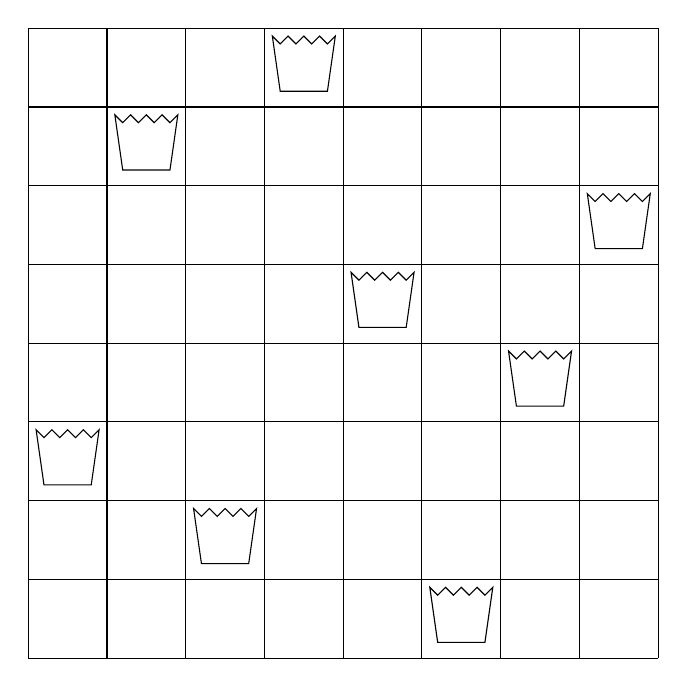
\begin{tikzpicture}
  []
  \foreach \i in {0,1,2,3,4,5,6,7,8} {
    \draw (0,\i) -- (8,\i);
    \draw (\i,0) -- (\i,8);
  }
  \draw (8,8) (0,0);
  \foreach \p in {(5,0), (2,1), (0,2), (6,3), (4,4), (7,5), (1,6), (3,7)}
  \draw \p +(0.2,0.2) -- +(0.8,0.2) -- +(0.9,0.9) -- +(0.8,0.8) -- +(0.7,0.9) -- +(0.6,0.8) -- +(0.5,0.9) -- +(0.4,0.8) -- +(0.3,0.9) -- +(0.2,0.8) -- +(0.1,0.9) -- cycle; 
\end{tikzpicture}
\end{figure}
<a name="%_fig_2.8"></a><div align=left><table width=100%><tr><td><img src="ch2-Z-G-23.gif" border="0">


</td></tr><caption align=bottom><div align=left><b>Figure 2.8:</b>  A solution to the eight-queens puzzle.</div></caption><tr><td>

</td></tr></table></div>
The ``eight-queens puzzle'' asks how to place eight queens on a
chessboard so that no queen is in check from any other (i.e., no two
queens are in the same row, column, or diagonal).  One possible
solution is shown in figure \ref{fig:2.8}.  One way to solve the
puzzle is to work across the board, placing a queen in each column.
Once we have placed $k - 1$ queens, we must place the $k$th queen in a
position where it does not check any of the queens already on the
board.  We can formulate this approach recursively: Assume that we
have already generated the sequence of all possible ways to place
$k - 1$ queens in the first $k - 1$ columns of the board.  For each of
these ways, generate an extended set of positions by placing a queen
in each row of the $k$th column.  Now filter these, keeping only
the positions for which the queen in the $k$th column is safe with
respect to the other queens.  This produces the sequence of all ways
to place $k$ queens in the first $k$ columns.  By continuing this
process, we will produce not only one solution, but all solutions to
the puzzle.


We implement this solution as a procedure \scheme|queens|, which returns
a sequence of all solutions to the problem of placing $n$ queens on an
$n \times n$ chessboard.  \scheme|Queens| has an internal procedure \scheme|queen-cols| that returns the sequence of all ways to place queens in
the first $k$ columns of the board.

\begin{schemedisplay}
(define (queens board-size)
  (define (queen-cols k)  
    (if (= k 0)
        (list empty-board)
        (filter
         (lambda (positions) (safe? k positions))
         (flatmap
          (lambda (rest-of-queens)
            (map (lambda (new-row)
                   (adjoin-position new-row k rest-of-queens))
                 (enumerate-interval 1 board-size)))
          (queen-cols (- k 1))))))
  (queen-cols board-size))
\end{schemedisplay}
In this procedure \scheme|rest-of-queens| is a way to place $k - 1$
queens in the first $k - 1$ columns, and \scheme|new-row| is a
proposed row in which to place the queen for the $k$th column.
Complete the program by implementing the representation for sets of
board positions, including the procedure \scheme|adjoin-position|,
which adjoins a new row-column position to a set of positions, and
\scheme|empty-board|, which represents an empty set of positions.  You
must also write the procedure \scheme|safe?|, which determines for a
set of positions, whether the queen in the $k$th column is safe with
respect to the others.  (Note that we need only check whether the new
queen is safe -- the other queens are already guaranteed safe with
respect to each other.)



\begin{Exercise}
\label{exc:2.43}
Louis Reasoner is having a terrible time doing exercise \ref{exc:2.42}.  His
\scheme|queens| procedure seems to work, but it runs extremely slowly.
(Louis never does manage to wait long enough for it to solve even the
$6 \times 6$ case.)  When Louis asks Eva Lu Ator for help, she points
out that he has interchanged the order of the nested mappings in the
\scheme|flatmap|, writing it as
\begin{schemedisplay}
(flatmap
 (lambda (new-row)
   (map (lambda (rest-of-queens)
          (adjoin-position new-row k rest-of-queens))
        (queen-cols (- k 1))))
 (enumerate-interval 1 board-size))
\end{schemedisplay}
Explain why this interchange makes the program run slowly.  Estimate
how long it will take Louis's program to solve the eight-queens
puzzle, assuming that the program in exercise \ref{exc:2.42} solves
the puzzle in time $T$.



\subsection{Example: A Picture Language}
\label{sec:2.2.4}



This section presents a simple language for drawing pictures that
illustrates the power of data abstraction and closure, and also
exploits higher-order procedures in an essential way.  The language is
designed to make it easy to experiment with patterns such as the ones
in figure \ref{fig:2.9}, which are composed of repeated elements that
are shifted and scaled.\footnote{22} In this language, the data
objects being combined are represented as procedures rather than as
list structure.  Just as \scheme|cons|, which satisfies the closure
property, allowed us to easily build arbitrarily complicated list
structure, the operations in this language, which also satisfy the
closure property, allow us to easily build arbitrarily complicated
patterns.

\begin{figure}
\placeholder{}
\caption{Designs generated with the picture language.}
\label{fig:2.9}
\end{figure}


\subsubsection*{The picture language}

When we began our study of programming in section \ref{sec:1.1}, we
emphasized the importance of describing a language by focusing on the
language's primitives, its means of combination, and its means of
abstraction.  We'll follow that framework here.

Part of the elegance of this picture language is that there is only
one kind of element, called a \textit{painter}.  A painter draws an
image that is shifted and scaled to fit within a designated
parallelogram-shaped frame.  For example, there's a primitive painter
we'll call \scheme|wave| that makes a crude line drawing, as shown in
figure \ref{fig:2.10}.  The actual shape of the drawing depends on the
frame -- all four images in figure \ref{fig:2.10} are produced by the
same \scheme|wave| painter, but with respect to four different frames.
Painters can be more elaborate than this: The primitive painter called
\scheme|rogers| paints a picture of MIT's founder, William Barton
Rogers, as shown in figure \ref{fig:2.11}.\footnote{23} The four
images in figure \ref{fig:2.11} are drawn with respect to the same
four frames as the \scheme|wave| images in figure \ref{fig:2.10}.


To combine images, we use various operations that construct new
painters from given painters.  For example, the \scheme|beside|
operation takes two painters and produces a new, compound painter that
draws the first painter's image in the left half of the frame and the
second painter's image in the right half of the frame.  Similarly,
\scheme|below| takes two painters and produces a compound painter that
draws the first painter's image below the second painter's image.
Some operations transform a single painter to produce a new painter.
For example, \scheme|flip-vert| takes a painter and produces a painter
that draws its image upside-down, and \scheme|flip-horiz| produces a
painter that draws the original painter's image left-to-right
reversed.

\begin{figure}
\centering
\placeholder
\caption{Images produced by the \scheme|wave| painter, with respect to
  four different frames.  The frames, shown with dotted lines, are not
  part of the images.}
\label{fig:2.10}
\end{figure}

\begin{figure}
  \centering
  \placeholder
  \caption{Images of William Barton Rogers, founder and first
    president of MIT, painted with respect to the same four frames as
    in figure \ref{fig:2.10} (original image reprinted with the
    permission of the MIT Museum).}
  \label{fig:2.11}
\end{figure}


Figure \ref{fig:2.12} shows the drawing of a painter called
\scheme|wave4| that is built up in two stages starting from \scheme|wave|:
\begin{schemedisplay}
(define wave2 (beside wave (flip-vert wave)))
(define wave4 (below wave2 wave2))
\end{schemedisplay}

\begin{figure}
  \centering
\placeholder
  \begin{schemedisplay}
    (define wave2                         (define wave4
      (beside wave (flip-vert wave)))       (below wave2 wave2))
  \end{schemedisplay}
  \caption{Creating a complex figure, starting from the \scheme|wave| painter of figure \ref{fig:2.10}.}
  \label{fig:2.12}
\end{figure}

In building up a complex image in this manner we are exploiting the
fact that painters are closed under the language's means of
combination.  The \scheme|beside| or \scheme|below| of two painters is
itself a painter; therefore, we can use it as an element in making
more complex painters.  As with building up list structure using \scheme|cons|, the closure of our data under the means of combination is
crucial to the ability to create complex structures while using only a
few operations.


Once we can combine painters, we would like to be able to abstract
typical patterns of combining painters.
We will implement the painter operations as Scheme procedures.
This means that we don't need a special abstraction mechanism
in the picture language:
Since the means of combination
are ordinary Scheme procedures, we automatically have the capability
to do anything with painter operations that we can do with
procedures.
For example, we can abstract the pattern in \scheme|wave4| as


\begin{schemedisplay}
(define (flipped-pairs painter)
  (let ((painter2 (beside painter (flip-vert painter))))
    (below painter2 painter2)))
\end{schemedisplay}
and define \scheme|wave4| as an instance of this pattern:


\begin{schemedisplay}
(define wave4 (flipped-pairs wave))
\end{schemedisplay}

We can also define recursive operations.
Here's one that makes painters split and branch
towards the right as shown in figures \ref{fig:2.13}
and  \ref{fig:2.14}:
\begin{schemedisplay}
(define (right-split painter n)
  (if (= n 0)
      painter
      (let ((smaller (right-split painter (- n 1))))
        (beside painter (below smaller smaller)))))
\end{schemedisplay}

<a name="%_fig_2.13"></a><div align=left><table width=100%><tr><td><div align=left><img src="ch2-Z-G-36.gif" border="0">
                   
<img src="ch2-Z-G-37.gif" border="0"> </div>

\begin{schemedisplay}
     right-split \textit{n}                   corner-split \textit{n}
\end{schemedisplay}
</td></tr><caption align=bottom><div align=left><b>Figure 2.13:</b>  Recursive plans for \scheme|right-split| and \scheme|corner-split|.</div></caption><tr><td>

</td></tr></table></div> 

We can produce balanced patterns by branching upwards
as well as towards the right (see exercise \ref{exc:2.44}
and figures \ref{fig:2.13} and  \ref{fig:2.14}):

\begin{schemedisplay}
(define (corner-split painter n)
  (if (= n 0)
      painter
      (let ((up (up-split painter (- n 1)))
            (right (right-split painter (- n 1))))
        (let ((top-left (beside up up))
              (bottom-right (below right right))
              (corner (corner-split painter (- n 1))))
          (beside (below painter top-left)
                  (below bottom-right corner))))))
\end{schemedisplay}

<a name="%_fig_2.14"></a><div align=left><table width=100%><tr><td><div align=left><img src="ch2-Z-G-38.gif" border="0">
          
<img src="ch2-Z-G-39.gif" border="0"> </div>

\begin{schemedisplay}
     (right-split wave 4)         (right-split rogers 4)
\end{schemedisplay}
<div align=left><img src="ch2-Z-G-40.gif" border="0">
          
<img src="ch2-Z-G-41.gif" border="0"> </div>

\begin{schemedisplay}
    (corner-split wave 4)         (corner-split rogers 4)
\end{schemedisplay}
</td></tr><caption align=bottom><div align=left><b>Figure 2.14:</b>  The recursive operations \scheme|right-split| and \scheme|corner-split| applied to the painters \scheme|wave| and \scheme|rogers|.
Combining four \scheme|corner-split| figures produces
symmetric \scheme|square-limit| designs as shown
in figure \ref{fig:2.9}.</div></caption><tr><td>

</td></tr></table></div> 

By placing four copies of a \scheme|corner-split|
appropriately, we obtain a pattern called \scheme|square-limit|, whose
application to \scheme|wave| and \scheme|rogers| is shown in
figure \ref{fig:2.9}:
\begin{schemedisplay}
(define (square-limit painter n)
  (let ((quarter (corner-split painter n)))
    (let ((half (beside (flip-horiz quarter) quarter)))
      (below (flip-vert half) half))))
\end{schemedisplay}

\begin{Exercise}
\label{exc:2.44}
Define the procedure \scheme|up-split| used by \scheme|corner-split|.
It is similar to \scheme|right-split|, except that it switches the
roles of \scheme|below| and \scheme|beside|.





\subsubsection*{Higher-order operations}


In addition to abstracting patterns of combining painters, we can work
at a higher level, abstracting patterns of combining painter operations.
That is, we can view the painter operations as elements to manipulate
and can write means of combination for these elements -- procedures that
take painter operations as arguments and create new painter operations.

For example, \scheme|flipped-pairs| and \scheme|square-limit| each
arrange four copies of a painter's image in a square pattern; they differ
only in how they orient the copies.
One way to abstract this pattern of painter combination is with
the following procedure, which takes four one-argument painter operations
and produces a painter operation that transforms a given
painter with those four operations and arranges the results in a square.
\scheme|Tl|, \scheme|tr|, \scheme|bl|, and \scheme|br| are the
transformations to apply to the top left copy, the top right copy,
the bottom left copy, and the bottom right copy, respectively.

\begin{schemedisplay}
(define (square-of-four tl tr bl br)
  (lambda (painter)
    (let ((top (beside (tl painter) (tr painter)))
          (bottom (beside (bl painter) (br painter))))
      (below bottom top))))
\end{schemedisplay}
Then \scheme|flipped-pairs| can be defined in terms
of \scheme|square-of-four| as follows:\footnote{24}

\begin{schemedisplay}
(define (flipped-pairs painter)
  (let ((combine4 (square-of-four identity flip-vert
                                  identity flip-vert)))
    (combine4 painter)))
\end{schemedisplay}
and \scheme|square-limit| can be expressed as\footnote{25}

\begin{schemedisplay}
(define (square-limit painter n)
  (let ((combine4 (square-of-four flip-horiz identity
                                  rotate180 flip-vert)))
    (combine4 (corner-split painter n))))
\end{schemedisplay}

\begin{Exercise}
\label{exc:2.45}
\scheme|Right-split| and \scheme|up-split| can be expressed as
instances of a general splitting operation.
Define a procedure \scheme|split| with the property that evaluating
\begin{schemedisplay}
(define right-split (split beside below))
(define up-split (split below beside))
\end{schemedisplay}
produces procedures \scheme|right-split| and \scheme|up-split| with the same
behaviors as the ones already defined.




\subsubsection*{Frames}


Before we can show how to implement painters and their
means of combination, we must first consider
frames.  A frame can be described by three vectors -- an origin vector
and two edge vectors.  The origin vector specifies the offset of the
frame's origin from some absolute origin in the plane, and the edge
vectors specify the offsets of the frame's corners from its origin.
If the edges are perpendicular, the frame will be rectangular.
Otherwise the frame will be a more general parallelogram.

Figure \ref{fig:2.15} shows a frame and its associated vectors.  In
accordance with data abstraction, we need not be
specific yet about how frames are represented, other than to say that
there is a constructor \scheme|make-frame|, which takes three vectors and
produces a frame, and three corresponding selectors \scheme|origin-frame|, \scheme|edge1-frame|, and \scheme|edge2-frame| (see
exercise \ref{exc:2.47}).

<a name="%_fig_2.15"></a><div align=left><table width=100%><tr><td><img src="ch2-Z-G-42.gif" border="0">
</td></tr><caption align=bottom><div align=left><b>Figure 2.15:</b>  A frame is described by three vectors -- an
origin and two edges.</div></caption><tr><td>

</td></tr></table></div> 

We will use coordinates in the unit square (0<u><</u> \textit{x},\textit{y}<u><</u> 1)
to specify images.
With each frame, we associate a \textit{frame coordinate map}, which
will be used to shift and scale images to fit the frame.  The map
transforms the unit square into the frame by
mapping the vector <strong>\textit{v}</strong> = (\textit{x},\textit{y}) to the vector sum
<div align=left><img src="ch2-Z-G-43.gif" border="0"></div>
For example, (0,0) is mapped to the origin of the frame, (1,1) to
the vertex diagonally opposite the origin, and (0.5,0.5) to the
center of the frame.  We can create a frame's coordinate map with the
following procedure:\footnote{26}

\begin{schemedisplay}
(define (frame-coord-map frame)
  (lambda (v)
    (add-vect
     (origin-frame frame)
     (add-vect (scale-vect (xcor-vect v)
                           (edge1-frame frame))
               (scale-vect (ycor-vect v)
                           (edge2-frame frame))))))
\end{schemedisplay}
Observe that applying \scheme|frame-coord-map| to a frame returns
a procedure that, given a vector, returns a vector.
If the argument vector is in the unit square, the result vector
will be in the frame.  For example,
\begin{schemedisplay}
((frame-coord-map a-frame) (make-vect 0 0))
\end{schemedisplay}
returns the same vector as
\begin{schemedisplay}
(origin-frame a-frame)
\end{schemedisplay}

\begin{Exercise}
\label{exc:2.46}
A two-dimensional vector <strong>v</strong> running from the origin to a point
can be represented as a pair
consisting of an \textit{x}-coordinate and a \textit{y}-coordinate.  Implement a data
abstraction for vectors by giving a constructor \scheme|make-vect| and
corresponding selectors \scheme|xcor-vect| and \scheme|ycor-vect|.  In
terms of your selectors and constructor, implement procedures \scheme|add-vect|, \scheme|sub-vect|, and \scheme|scale-vect| that perform
the operations vector addition, vector subtraction, and multiplying a
vector by a scalar:
<div align=left><img src="ch2-Z-G-44.gif" border="0"></div>


\begin{Exercise}
\label{exc:2.47}
Here are two possible constructors for frames:
\begin{schemedisplay}
(define (make-frame origin edge1 edge2)
  (list origin edge1 edge2))

(define (make-frame origin edge1 edge2)
  (cons origin (cons edge1 edge2)))
\end{schemedisplay}
For each constructor supply the appropriate selectors to produce an
implementation for frames.




\subsubsection*{Painters}


A painter is represented as a procedure that, given a frame
as argument, draws a particular image shifted and scaled to fit the frame.
That is to say, if \scheme|p| is a painter and \scheme|f| is a frame, then we
produce \scheme|p|'s image in \scheme|f| by calling \scheme|p| with \scheme|f| as
argument.

The details of how primitive painters are implemented depend on the
particular characteristics of the graphics system and the type of
image to be drawn.  For instance, suppose we have a procedure \scheme|draw-line| that draws a line on the screen between two specified
points.  Then we can create painters for line drawings, such as the
\scheme|wave| painter in figure \ref{fig:2.10}, from lists of line
segments as follows:\footnote{27}\begin{schemedisplay}
(define (segments->painter segment-list)
  (lambda (frame)
    (for-each
     (lambda (segment)
       (draw-line
        ((frame-coord-map frame) (start-segment segment))
        ((frame-coord-map frame) (end-segment segment))))
     segment-list)))
\end{schemedisplay}
The segments are given using coordinates with respect to the unit
square.  For each segment in the list, the painter transforms the
segment endpoints with the frame coordinate map and draws a line
between the transformed points.

Representing painters as procedures erects a powerful abstraction
barrier in the picture language.  We can create and intermix
all sorts of primitive painters, based on a variety of graphics
capabilities. The details of their implementation do not matter.  Any
procedure can serve as a painter, provided that it takes a frame as
argument and draws something scaled to fit the frame.\footnote{28}

\begin{Exercise}
\label{exc:2.48}
A directed line segment in the
plane can be represented as a pair of vectors -- the
vector running from the origin to the start-point of the segment, and
the vector running from the origin to the end-point of the segment.
Use your vector representation from exercise \ref{exc:2.46} to
define a representation for segments with a constructor \scheme|make-segment| and selectors \scheme|start-segment| and \scheme|end-segment|.



\begin{Exercise}
\label{exc:2.49}
Use \scheme|segments->painter| to define the following primitive painters:

a.  The painter that draws the outline of the designated frame.

b.  The painter that draws an ``X'' by connecting opposite corners of
the frame.

c.  The painter that draws a diamond shape by connecting the midpoints of
the sides of the frame.

d.  The \scheme|wave| painter.




\subsubsection*{Transforming and combining painters}


An operation on painters (such as \scheme|flip-vert| or \scheme|beside|)
works by creating a painter that invokes the original painters
with respect to frames derived from the argument frame.
Thus, for example, \scheme|flip-vert| doesn't have to know how a painter
works in order to flip it -- it just has to know how to turn a frame
upside down:
The flipped painter just uses the original painter,
but in the inverted frame.

Painter operations are based on
the procedure \scheme|transform-painter|, which takes as arguments a painter and
information on how to transform a frame and
produces a new painter.  The transformed painter, when called on a frame,
transforms the frame and
calls the original painter on the transformed frame.
The arguments to \scheme|transform-painter| are points (represented as vectors)
that specify the corners of the new frame:
When mapped into
the frame, the first point specifies the new frame's origin
and the other two specify the ends of its edge vectors.
Thus, arguments within the
unit square specify a frame contained within the original frame.

\begin{schemedisplay}
(define (transform-painter painter origin corner1 corner2)
  (lambda (frame)
    (let ((m (frame-coord-map frame)))
      (let ((new-origin (m origin)))
        (painter
         (make-frame new-origin
                     (sub-vect (m corner1) new-origin)
                     (sub-vect (m corner2) new-origin)))))))
\end{schemedisplay}

Here's how to flip painter images vertically:
\begin{schemedisplay}
(define (flip-vert painter)
  (transform-painter painter
                     (make-vect 0.0 1.0)   \textit{; new \scheme|origin|}
                     (make-vect 1.0 1.0)   \textit{; new end of \scheme|edge1|}
                     (make-vect 0.0 0.0))) \textit{; new end of \scheme|edge2|}
\end{schemedisplay}
Using \scheme|transform-painter|, we can easily define new transformations.
For example, we can define a painter that shrinks its image to the
upper-right quarter of the frame it is given:
\begin{schemedisplay}
(define (shrink-to-upper-right painter)
  (transform-painter painter
                     (make-vect 0.5 0.5)
                     (make-vect 1.0 0.5)
                     (make-vect 0.5 1.0)))
\end{schemedisplay}
Other transformations rotate images counterclockwise by 90 degrees\footnote{29}
\begin{schemedisplay}
(define (rotate90 painter)
  (transform-painter painter
                     (make-vect 1.0 0.0)
                     (make-vect 1.0 1.0)
                     (make-vect 0.0 0.0)))
\end{schemedisplay}
or squash images towards the center of the frame:\footnote{30}
\begin{schemedisplay}
(define (squash-inwards painter)
  (transform-painter painter
                     (make-vect 0.0 0.0)
                     (make-vect 0.65 0.35)
                     (make-vect 0.35 0.65)))
\end{schemedisplay}

Frame transformation is also the key to
defining means of combining two or more painters.
The \scheme|beside| procedure,
for example, takes two painters, transforms them
to paint in the left and right halves of an argument frame respectively,
and produces a new, compound painter.
When the compound painter is given a frame, it
calls the first transformed painter to paint in the left half of
the frame and calls the second transformed painter to paint in the
right half of the frame:
\begin{schemedisplay}
(define (beside painter1 painter2)
  (let ((split-point (make-vect 0.5 0.0)))
    (let ((paint-left
           (transform-painter painter1
                              (make-vect 0.0 0.0)
                              split-point
                              (make-vect 0.0 1.0)))
          (paint-right
           (transform-painter painter2
                              split-point
                              (make-vect 1.0 0.0)
                              (make-vect 0.5 1.0))))
      (lambda (frame)
        (paint-left frame)
        (paint-right frame)))))
\end{schemedisplay}

Observe how the painter data abstraction, and in particular the
representation of painters as procedures, makes \scheme|beside| easy to
implement.  The \scheme|beside| procedure need not know anything
about the details of the component painters other than that each
painter will draw something in its designated frame.

\begin{Exercise}
\label{exc:2.50}
Define the transformation \scheme|flip-horiz|, which flips
painters horizontally, and transformations that rotate
painters counterclockwise by 180 degrees and 270 degrees.



\begin{Exercise}
\label{exc:2.51}
Define the \scheme|below| operation for painters.  \scheme|Below| takes two
painters as arguments.  The resulting painter, given a frame,
draws with the first painter in the
bottom of the frame and with the second painter in the top.  Define \scheme|below| in two different ways -- first by writing a procedure that is
analogous to the \scheme|beside| procedure given above, and
again in terms of \scheme|beside| and suitable
rotation operations (from exercise \ref{exc:2.50}).




\subsubsection*{Levels of language for robust design}

The picture language exercises some of the critical ideas
we've introduced about abstraction with procedures and data.  The
fundamental data abstractions, painters, are implemented using
procedural representations, which enables the language to
handle different basic drawing capabilities in a uniform way.  The
means of combination satisfy the closure property, which permits us to
easily build up complex designs.  Finally, all the tools for
abstracting procedures are available to us for abstracting means of
combination for painters.


We have also obtained a glimpse of another crucial idea about
languages and program design.  This is the approach of <em>stratified
design</em>, the notion that a complex system should be structured as a
sequence of levels that are described using a sequence of languages.
Each level is constructed by combining parts that are regarded as
primitive at that level, and the parts constructed at each level are
used as primitives at the next level.  The language used at each level
of a stratified design has primitives, means of combination, and means
of abstraction appropriate to that level of detail.

Stratified design pervades the engineering of complex systems.  For
example, in computer engineering, resistors and transistors are
combined (and described using a language of analog circuits) to
produce parts such as and-gates and or-gates, which form the
primitives of a language for digital-circuit design.\footnote{31}
These parts are combined to build
processors, bus structures, and memory systems, which are in turn
combined to form computers, using languages appropriate to computer
architecture.  Computers are combined to form distributed systems,
using languages appropriate for describing network interconnections,
and so on.

As a tiny example of stratification, our picture language uses
primitive elements (primitive painters) that are created using a
language that specifies points and lines to provide the lists of line
segments for \scheme|segments->painter|, or the
shading details for a painter like \scheme|rogers|.  The bulk of our
description of the picture language focused on combining these
primitives, using geometric combiners such as \scheme|beside| and \scheme|below|.  We also worked at a higher level, regarding \scheme|beside| and
\scheme|below| as primitives to be manipulated in a language whose
operations, such as \scheme|square-of-four|, capture common patterns of
combining geometric combiners.

Stratified design helps make programs \textit{robust}, that is, it makes
it likely that small changes in a specification will require
correspondingly small changes in the program.  For instance, suppose
we wanted to change the image based on \scheme|wave| shown in
figure \ref{fig:2.9}.  We could work at the lowest level
to change the detailed appearance of the \scheme|wave| element; we could
work at the middle level to change the way \scheme|corner-split|
replicates the \scheme|wave|; we could work at the highest level to
change how \scheme|square-limit| arranges the four copies of the corner.
In general, each level of a stratified design provides a different
vocabulary for expressing the characteristics of the system, and a
different kind of ability to change it.

\begin{Exercise}
\label{exc:2.52}
Make changes to the square limit of \scheme|wave| shown in
figure \ref{fig:2.9} by working at each of the levels
described above.  In particular:

a.  Add some segments to the primitive \scheme|wave| painter
of exercise  \ref{exc:2.49} (to add a smile, for example).

b.  Change the pattern constructed by \scheme|corner-split|
(for example, by using only one copy of the
\scheme|up-split| and \scheme|right-split| images instead of two).

c.  Modify the version of \scheme|square-limit| that uses \scheme|square-of-four|
so as to assemble the corners in a different pattern.  (For example, you
might make the big Mr. Rogers look outward from each corner of the square.)


<div class=smallprint><hr></div>
% Footnote 6
The use of the word ``closure'' here comes from abstract algebra,
where a set of elements is said to be closed under an operation if
applying the operation to elements in the set produces an element that
is again an element of the set.  The Lisp community
also (unfortunately) uses the word ``closure'' to describe a totally unrelated
concept: A closure is an implementation technique for representing
procedures with free variables.  We do not use the word ``closure'' in
this second sense in this book.

% Footnote 7
The notion that a means of
combination should satisfy closure is a straightforward idea.
Unfortunately, the data combiners provided in many popular programming
languages do not satisfy closure, or make closure cumbersome to
exploit.  In Fortran or Basic, one typically combines data elements by
assembling them into arrays -- but one cannot form arrays whose
elements are themselves arrays.  Pascal and C admit structures whose
elements are structures.  However, this requires that the programmer
manipulate pointers explicitly, and adhere to the restriction that
each field of a structure can contain only elements of a prespecified form.
Unlike
Lisp with its pairs, these languages have no built-in general-purpose
glue that makes it easy to manipulate compound data in a uniform way.
This limitation lies behind Alan Perlis's comment in his foreword to
this book: ``In Pascal the plethora of declarable data structures
induces a specialization within functions that inhibits and penalizes
casual cooperation.  It is better to have 100 functions operate on one
data structure than to have 10 functions operate on 10 data
structures.''

% Footnote 8
In this book, we use \textit{list} to mean a chain of
pairs terminated by the end-of-list marker.  In contrast, the term
\textit{list structure} refers to any data structure made out of pairs,
not just to lists.

% Footnote 9
Since nested applications of \scheme|car| and \scheme|cdr|
are cumbersome to write, Lisp dialects provide abbreviations for
them -- for instance,
<div align=left><img src="ch2-Z-G-14.gif" border="0"></div>
The names of all such procedures start with \scheme|c| and end with \scheme|r|.  Each \scheme|a| between them stands for a \scheme|car| operation and
each \scheme|d| for a \scheme|cdr| operation, to be applied in the same order
in which they appear in the name.  The names \scheme|car| and \scheme|cdr|
persist because simple combinations like \scheme|cadr| are
pronounceable.

% Footnote 10
It's remarkable how much energy in the
standardization of Lisp dialects has been dissipated in arguments that
are literally over nothing: Should \scheme|nil| be an ordinary name?
Should the value of \scheme|nil| be a symbol?  Should it be a list?
Should it be a pair?  In Scheme, \scheme|nil| is an ordinary name,
which we use in this section as a variable whose value is
the end-of-list marker (just as \scheme|true| is an ordinary variable
that has a true value).  Other dialects of
Lisp, including Common Lisp, treat \scheme|nil| as a special symbol.  The
authors of this book, who have endured too many language
standardization brawls, would like to avoid the entire issue.  Once we
have introduced quotation in section \ref{sec:2.3}, we will
denote the empty list as \scheme|'()| and dispense with the
variable \scheme|nil| entirely.

% Footnote 11
To define \scheme|f| and \scheme|g| using
\scheme|lambda| we would write
\begin{schemedisplay}
(define f (lambda (x y . z) <\textit{body}>))
(define g (lambda w <\textit{body}>))
\end{schemedisplay}

% Footnote 12
Scheme
standardly provides a \scheme|map| procedure that is more general
than the one described here.
This more general \scheme|map|
takes a procedure of \textit{n} arguments, together with \textit{n} lists, and
applies the procedure to all the first elements of
the lists, all the second elements of the lists, and so on,
returning a list of the results.  For example:
\begin{schemedisplay}
(map + (list 1 2 3) (list 40 50 60) (list 700 800 900))
<i>(741 852 963)</i>

(map (lambda (x y) (+ x (* 2 y)))
     (list 1 2 3)
     (list 4 5 6))
<i>(9 12 15)</i>
\end{schemedisplay}



% Footnote 13
The order of the
first two clauses in the \scheme|cond| matters, since the empty list
satisfies \scheme|null?| and also is not a pair.

% Footnote 14
This is, in fact, precisely the \scheme|fringe| procedure from
exercise \ref{exc:2.28}.  Here we've renamed it to emphasize that
it is part of a family of general sequence-manipulation procedures.

% Footnote 15
Richard Waters (1979)
developed a program that automatically analyzes traditional Fortran
programs, viewing them in terms of maps, filters, and accumulations.
He found that fully 90 percent of the code in the Fortran Scientific
Subroutine Package fits neatly into this paradigm.  One of the reasons
for the success of Lisp as a programming language is that lists
provide a standard medium for expressing ordered collections so that
they can be manipulated using higher-order operations.  The
programming language APL owes much of its power and appeal to a
similar choice. In APL all data are represented as arrays, and there is a
universal and convenient set of generic operators for all sorts of
array operations.

% Footnote 16
According to Knuth (1981), this rule was formulated by
W. G. Horner early in the nineteenth century, but the method was
actually used by Newton over a hundred years earlier.  Horner's rule
evaluates the polynomial using fewer additions and multiplications
than does the straightforward method of first computing \textit{a}<sub>\textit{n}</sub> \textit{x}<sup>\textit{n}</sup>,
then adding \textit{a}<sub>\textit{n}-1</sub>\textit{x}<sup>\textit{n}-1</sup>, and so on.  In fact, it is possible to
prove that any algorithm for evaluating arbitrary polynomials must use
at least as many additions and multiplications as does Horner's rule,
and thus Horner's rule is an optimal algorithm for polynomial
evaluation.  This was proved (for the number of additions) by
A. M. Ostrowski in a 1954 paper that essentially founded the modern
study of optimal algorithms.  The analogous statement for
multiplications was proved by V. Y. Pan in 1966.  The book by Borodin
and Munro (1975) provides an overview of these and other results about
optimal algorithms.

% Footnote 17
This definition uses the
extended version of \scheme|map| described in footnote <a href="#footnote_Temp_166">12</a>.

% Footnote 18
This approach to nested mappings was shown
to us by David Turner, whose languages KRC and Miranda provide elegant
formalisms for dealing with these constructs.  The examples in this
section (see also exercise \ref{exc:2.42}) are adapted from Turner
1981.  In section \ref{sec:3.5.3}, we'll see how this
approach generalizes to infinite sequences.

% Footnote 19
We're
representing a pair here as a list of two elements rather than as a
Lisp pair.  Thus, the ``pair'' (\textit{i},\textit{j}) is represented as \begin{schemedisplay}
(list i
j)\end{schemedisplay}, not \scheme|(cons i j)|.

% Footnote 20
The set \textit{S} - \textit{x} is the set of all elements
of \textit{S}, excluding \textit{x}.

% Footnote 21
Semicolons in Scheme code are used to
introduce \textit{comments}.  Everything from the semicolon to the end of
the line is ignored by the interpreter.  In this book we don't use
many comments; we try to make our programs self-documenting by using
descriptive names.

% Footnote 22
The picture language is based on the language
Peter Henderson created to construct
images like M.C. Escher's ``Square Limit'' woodcut (see Henderson 1982).
The woodcut incorporates a
repeated scaled pattern, similar to the arrangements drawn using
the \scheme|square-limit| procedure in this section.

% Footnote 23
William Barton Rogers (1804-1882) was the founder and first president
of MIT.  A geologist and talented teacher, he taught at William and
Mary College and at the University of Virginia.  In 1859 he moved to
Boston, where he had more time for research, worked on a plan
for establishing a ``polytechnic institute,'' and served as
Massachusetts's first State Inspector of Gas Meters.

When MIT was established in 1861, Rogers was elected its first
president.  Rogers espoused an ideal of ``useful learning'' that was
different from the university education of the time, with its
overemphasis on the classics, which, as he wrote, ``stand in the way of
the broader, higher and more practical instruction and discipline of
the natural and social sciences.''  This education was likewise to be
different from narrow trade-school education.  In Rogers's words:
<blockquote>
The world-enforced distinction between the practical and the
scientific worker is utterly futile, and the whole experience of
modern times has demonstrated its utter worthlessness.
</blockquote>

Rogers served as president of MIT until 1870, when he resigned due to
ill health.  In 1878 the second president of MIT, John Runkle,
resigned under the pressure of a financial crisis brought on by the
Panic of 1873 and strain of fighting off attempts by Harvard to take
over MIT.  Rogers returned to hold the office of president until
1881.

Rogers collapsed and died while addressing MIT's graduating class at
the commencement exercises of 1882.  Runkle quoted Rogers's last
words in a memorial address delivered that same year:
<blockquote>
``As I stand here today and see what the Institute is, \scheme|...| I call
to mind the beginnings of science.  I remember one hundred and fifty
years ago Stephen Hales published a pamphlet on the subject of
illuminating gas, in which he stated that his researches had
demonstrated that 128 grains of bituminous coal -- ''
``Bituminous coal,'' these were his last words on earth.  Here he bent
forward, as if consulting some notes on the table before him, then
slowly regaining an erect position, threw up his hands, and was
translated from the scene of his earthly labors and triumphs to ``the
tomorrow of death,'' where the mysteries of life are solved, and the
disembodied spirit finds unending satisfaction in contemplating the
new and still unfathomable mysteries of the infinite future.
</blockquote>
In the words of  Francis A. Walker
(MIT's third president):
<blockquote>
All his life he had borne himself most faithfully and heroically, and
he died as so good a knight would surely have wished, in harness, at
his post, and in the very part and act of public duty.
</blockquote>

% Footnote 24
Equivalently, we could
write
\begin{schemedisplay}
(define flipped-pairs
  (square-of-four identity flip-vert identity flip-vert))
\end{schemedisplay}


% Footnote 25
\scheme|Rotate180|
rotates a painter by 180 degrees (see exercise \ref{exc:2.50}).
Instead of \scheme|rotate180| we could say \scheme|(compose flip-vert flip-horiz)|, using
the \scheme|compose| procedure from exercise \ref{exc:1.42}.

% Footnote 26
\scheme|Frame-coord-map| uses
the vector operations described in exercise \ref{exc:2.46} below, which we
assume have been implemented using some representation for vectors.
Because of data abstraction, it doesn't matter what this vector
representation is, so long as the vector operations behave correctly.

% Footnote 27
\scheme|Segments->painter| uses the representation for line
segments described in exercise \ref{exc:2.48} below.
It also uses the \scheme|for-each| procedure described in exercise \ref{exc:2.23}.

% Footnote 28
For example, the \scheme|rogers| painter of
figure \ref{fig:2.11} was constructed from a gray-level image.
For each point in a given frame,
the \scheme|rogers| painter determines the point in the image that is mapped to it
under the frame coordinate map, and shades it
accordingly.  By allowing different types of painters, we are capitalizing on the
abstract data idea discussed in section \ref{sec:2.1.3}, where we
argued that a rational-number representation could be anything at all that
satisfies an appropriate condition.  Here we're using the fact that a
painter can be implemented in any way at all, so long as it draws
something in the designated frame.  Section \ref{sec:2.1.3} also
showed how pairs could be implemented as procedures.  Painters are our
second example of a procedural representation for data.

% Footnote 29
\scheme|Rotate90| is a pure rotation only for square
frames, because it also stretches and shrinks the image to fit into
the rotated frame.

% Footnote 30
The diamond-shaped images in figures \ref{fig:2.10}
and \ref{fig:2.11} were created with \scheme|squash-inwards| applied to
\scheme|wave| and \scheme|rogers|.

% Footnote 31
Section \ref{sec:3.3.4} describes one such language.

</div>

